%===================================================================================
% PREÁMBULO
%-----------------------------------------------------------------------------------
\documentclass[a4paper,10pt,twocolumn]{article}

%===================================================================================
% Paquetes
%-----------------------------------------------------------------------------------
\usepackage{amsmath}
\usepackage{amsfonts}
\usepackage{algorithm}
\usepackage{algorithmic}
\usepackage{amssymb}
\usepackage{informe}
\usepackage{lipsum}
\usepackage[utf8]{inputenc}
\usepackage{listings}
\usepackage{algorithmic}
\usepackage[pdftex]{hyperref}
%-----------------------------------------------------------------------------------
% Configuración
%-----------------------------------------------------------------------------------
\hypersetup{colorlinks,%
	    citecolor=black,%
	    filecolor=black,%
	    linkcolor=black,%
	    urlcolor=blue}

%===================================================================================



%===================================================================================
% Presentacion
%-----------------------------------------------------------------------------------
% Título
%-----------------------------------------------------------------------------------
\title{Simulaci\'on de Agentes}

%-----------------------------------------------------------------------------------
% Autores
%-----------------------------------------------------------------------------------
\author{\\
	\name Carlos Rafael Ortega Lezcano \\ \addr Grupo C411 }


%-----------------------------------------------------------------------------------
% Tutores
%-----------------------------------------------------------------------------------
%\tutors{\\}

%-----------------------------------------------------------------------------------
% Headings
%-----------------------------------------------------------------------------------
%\jcematcomheading{\the\year}{1-\pageref{end}}{Carlos Rafael}

%-----------------------------------------------------------------------------------
%\ShortHeadings{Simulacio\'n basada en Eventos Discretos}{Carlos Rafael}
%===================================================================================



%===================================================================================
% DOCUMENTO
%-----------------------------------------------------------------------------------
\begin{document}

%-----------------------------------------------------------------------------------
% NO BORRAR ESTA LINEA!
%-----------------------------------------------------------------------------------
\twocolumn[
%-----------------------------------------------------------------------------------

\maketitle

%===================================================================================
% Resumen y Abstract
%-----------------------------------------------------------------------------------
\selectlanguage{spanish} % Para producir el documento en Español

%-----------------------------------------------------------------------------------
% Palabras clave
%-----------------------------------------------------------------------------------
%\begin{keywords}
%	Separadas,
%	Por,
%	Comas.
%\end{keywords}

%-----------------------------------------------------------------------------------
% Temas
%-----------------------------------------------------------------------------------
%\begin{topics}
%	Tema, Subtema.
%\end{topics}


%-----------------------------------------------------------------------------------
% NO BORRAR ESTAS LINEAS!
%-----------------------------------------------------------------------------------
\vspace{0.8cm}
]
%-----------------------------------------------------------------------------------


%===================================================================================

%===================================================================================

\section*{Orden del Problema}

El ambiente en el cual intervienen los agentes es discreto y tiene la forma de un rectangulo de N x M. El ambiente es de informacion completa, por tanto todos los agentes conocen toda la informacion sobre el agente. El ambiente puede varıar aleatoriamente cada t unidades de tiempo. El valor de t es conocido. Las acciones que realizan los agentes ocurren por turnos. En un turno, los agentes realizan sus acciones, una sola por cada agente, y modifican el medio sin que este varie a no ser que cambie por una accion de los agentes. En el siguiente, el ambiente puede variar. Si es el momento de cambio del ambiente, ocurre primero el cambio natural del ambiente y luego la variacion aleatoria. En una unidad de tiempo ocurren el turno del agente y el turno de cambio del ambiente. Los elementos que pueden existir en el ambiente son obstaculos, suciedad, ni\~nos, el corral y los agentes que son llamados Robots de Casa. A continuacion se precisan las caracterısticas de los elementos del ambiente:

\begin{enumerate}
	\item[] \textbf{Obstaculos}: estos ocupan una unica casilla en el ambiente. Ellos pueden ser movidos, empujandolos, por los ni\~nos, una unica casilla. El Robot de Casa sin embargo no puede moverlo. No pueden ser movidos ninguna de las casillas ocupadas por cualquier otro elemento del ambiente.

	\item[] \textbf{Suciedad}: la suciedad es por cada casilla del ambiente. Solo puede aparecer en casillas que previamente estuvieron vacıas. Esta, o aparece en el estado inicial o es creada por los ni\~nos.

	\item[] \textbf{Corral}: el corral ocupa casillas adyacentes en numero igual al del total de ni\~nos presentes en el ambiente. El corral no puede moverse. En una casilla del corral solo puede coexistir un ni\~no. En una casilla del corral, que este vacıa, puede entrar un robot. En una misma casilla del corral pueden coexistir un ni\~no y un robot solo si el robot lo carga, o si acaba de dejar al ni\~no.

	\item[] \textbf{Ni\~no}: los ni\~nos ocupan solo una casilla. Ellos en el turno del ambiente se mueven, si es posible (si la casilla no esta ocupada: no tiene suciedad, no esta el corral, no hay un Robot de Casa), y aleatoriamente (puede que no ocurra movimiento), a una de las casilla adyacentes. Si esa casilla esta ocupada por un obstaculo este es empujado por el ni\~no, si en la direccion hay mas de un obstaculo, entonces se desplazan todos. Si el obstaculo esta en una posicion donde no puede ser empujado y el ni\~no lo intenta, entonces el obstaculo no se mueve y el ni\~no ocupa la misma posicion. Los ni\~nos son los responsables de que aparezla suciedad. Si en una cuadrıcula de 3 por 3 hay un solo ni\~no, entonces, luego de que el se mueva aleatoriamente, una de las casillas de la cuadrıcula anterior que este vacıa puede haber sido ensuciada. Si hay dos ni\~nos se pueden ensuciar hasta 3. Si hay tres ni\~nos o mas pueden resultar sucias hasta 6. Los ni\~nos cuando estan en una casilla del corral, ni se mueven ni ensucian. Si un ni\~no es capturado por un Robot de Casa tampoco se mueve ni ensucia.

	\item[] \textbf{Robot de Casa}: El Robot de Casa se encarga de limpiar y de controlar a los ni\~nos. El Robot se mueve a una de las casillas adyacentee, las que decida. Solo se mueve una casilla sino carga un ni\~no. Si carga un ni\~no pude moverse hasta dos casillas consecutivas. Tambien puede realizar las acciones de limpiar y cargar ni\~nos. Si se mueve a una casilla con suciedad, en el proximo turno puede decidir limpiar o moverse. Si se mueve a una casilla donde esta un ni\~no, inmediatamente lo carga. En ese momento, coexisten en la casilla Robot y ni\~no. Si se mueve a una casilla del corral que esta vacıa, y carga un ni\~no, puede decidir si lo deja esta casilla o se sigue moviendo. El Robot puede dejar al ni\~no que carga en cualquier casilla. En ese momento cesa el movimiento del Robot en el turno, y coexisten hasta el proximo turno, en la misma casilla, Robot y ni\~no.

\end{enumerate}


\section*{Ideas seguidas para la soluci\'on del Problema}

Se defini\'o el ambiente en el cual nuestro agente realizar\'a sus tareas. Este se defini\'o empleando las condiciones impuestas en el problema, el ambiente tiene dos importantes funcionalidades: \textbf{remake} y \textbf{next}. Como es necesario cada $t$ turnos realizar una reorganizaci\'on del ambiente entonces las entitades que intervienen en el ambiente son objetos los cuales mantienen un estado acorde a su interacci\'on con otras entidades (por ejemplo un corral que tiene un ni\~no dentro luego de una reorganizaci\'on continuar\'a teniendo la misma instancia asociada). De esta forma podemos describir de una forma m\'as exacta las acciones del robot y los ni\~nos en el ambiente. Para avanzar al pr\'oximo estado del ambiente se realiza \text{next} este computa los movimientos de las entidades del ambiente adem\'as de la generaci\'on de basura y el movimiento de objetos, de esta forma describimos el cambio natural del ambiente.

Contamos con dos tipos de agentes, los cuales se diferencian en la forma que interpretan el ambiente y las prioridades que tiene a la hora de lograr el objetivo. Los agentes definen 3 funciones b\'asicas: \textbf{next}, \textbf{see} y \textbf{action}. Para ambos agentes \textbf{action} ser\'a la misma ya que describe que acciones hace de acuerdo a su interacci\'on con las entidades. Es importante aclarar que siempre que le sea posible limpiar una casilla en la que se encuentre lo har\'a, no ignorar\'a esta casilla, de esta forma siempre se intenta reducir el porciento de basura en caso que se realice otra acci\'on. La definici\'on para el conjunto de acciones y prioridades que da el robot.

\begin{algorithm}
	\begin{algorithmic}
		\STATE Action (env):
		\STATE $\;\;\;$ bot.looked $\leftarrow$ Entidad seleccionada por el bot
		\STATE $\;\;\;$ x, y $\leftarrow$ bot.position 
		\STATE $\;\;\;$ \textbf{if} env[x, y].dirty \textbf{then} bot.clean
		\STATE $\;\;\;$ \textbf{if} env[x, y].cradle and bot.carry \textbf{then} bot.drop
		\STATE $\;\;\;$ \textbf{if} bot.looked \textbf{is} child \textbf{then} bot.catch\_child
		\STATE $\;\;\;$ \textbf{if} bot.looked \textbf{then} bot.move\_to\_entity
		\STATE $\;\;\;$ bot.stop
	\end{algorithmic}
\end{algorithm}

Como podemos ver el robot primeramente intentar\'a limpiar la casilla en la que se encuentra si esta se ensucia y termina su turno, en caso de estar cargando un ni\~no y encontrarse en un corral deja el ni\~no, el robot tiene un atributo \textbf{looked} el cual representa la entidad a la cual le presto atenci\'on cuando analiz\'o el ambiente, en caso que sea un ni\~no significa que no tiene carga por lo tanto intentar\'a recogerlo para reducir la basura generada y tener un paso extra, si por otra parte contempla una cuna o una casilla sucia intentar\'a llegar a esta por el camino m\'as corto posible. Este esquema es muy parecido a la arquitectura de Brooks vista en [1].

\section*{Modelo de Agentes}

Como se expuso anteriormente la diferencia en los modelos empleados radica en como el agente considera las prioridades a la hora de realizar las tareas. Para el problema se consideraron 2 modelos, ambos tienen en com\'un que siempre que el robot llegue a una casilla sucia la limpiar\'a en el pr\'oximo turno, el robot siempre intentar\'a tener un ni\~no para maximizar la cantidad de pasos que puede dar\\

\textbf{Modelo 1}: Este modelo realizar\'a la acci\'on m\'as cercana posible, si tiene m\'as cerca una cuna vac\'ia entonces dejar\'a al ni\~no, si tiene una basura m\'as cerca, se mover\'a a limpiarla, este modelo sigue una concepci\'on similar a los agentes reactivos, contempla el ambiente y realiza una acci\'on sin observar las consecuencias que tendr\'a sus acciones, en este caso el agente no tiene memoria por lo tanto es puro, reacciona a cada cambio del ambiente.\\

La funci\'on \textbf{see}, que define el comportamiento del agente acorde a lo que tiene en el ambiente es:

\begin{algorithm}
	\begin{algorithmic}
		\STATE See (env):
		\STATE $\;\;\;$ \textbf{if} \textbf{not} bot.carry \textbf{then} bot.search\_child
		\STATE $\;\;\;$ \textbf{else} near\{{bot.seach\_cradle} \textbf{or} bot.seach\_cradle\}
	\end{algorithmic}
\end{algorithm}

En este caso siempre intentamos cargar un ni\~no, en caso de tenerlo buscamos lo m\'as cercano al robot, el corral o una casilla sucia.\\

\textbf{Modelo 2}: Este modelo va m\'as enfocado en ganar, por lo tanto su objetivo es buscar a los ni\~nos y ponerlos en el corral, este modelo no lo consideramos proactivo, ya que aunque tome la iniciativa para buscar limpiar toda la casa, no consider\'a que tan pr\'oximo este del despido para tomar acciones con respecto a esto. 

\begin{algorithm}
	\begin{algorithmic}
		\STATE See (env):
		\STATE $\;\;\;$ \textbf{if} \textbf{not} bot.carry \textbf{then} bot.search\_child
		\STATE $\;\;\;$ \textbf{if} bot.carry \textbf{then} bot.search\_cradle
		\STATE $\;\;\;$ bot.seach\_trash
	\end{algorithmic}
\end{algorithm}

En este caso el robot busca igual que el primero tomar un ni\~no y pero ahora siempre lo mover\'a a la cuna disponible, de esta forma intentar\'a primero recoger a todos los ni\~nos e ir\'a limpiando la basura a medida que se mueve.

Adicionalmente se implement\'o otro modelo, el cual intenta recoger a todos los ni\~nos pero en caso que su acci\'on pueda generar un aumento al 50\% de basura en el ambiente, dar\'a m\'as prioridad a limpiar el ambiente para no ser despedido. 

Es importante aclarar que el robot y los ni\~nos se mueven en las 8 direcciones, adem\'as que a primera vista se aprecia que en caso que la tarea de recoger un ni\~no primero se dificulta excesivamente el robot siempre ser\'a despedido ya que en ambos modelos es una prioridad buscar un ni\~no, para ello se realiz\'o otro agente que busca igualar todas las tareas en cuanto al tipo de entidad detectada, pero continuando dando prioridad a las m\'as cercanas.

\section*{Simulaciones Realizadas}

Se generar\'on 10 ambientes para cada uno se hizo 30 corridas usando cada modelo de agente (los 2 principales expuestos). Al analizar los resultados podemos concluir que el segundo modelo fue mejor para resover el problema, incluso las veces que no puedo completar la tarea y fue despedido no dejo una cantidad grande de basura en el ambiente. Si observamos los ambientes generados podemos ver como existen algunos que por sus caracter\'isticas ser\'an muy f\'aciles para el robot o no habr\'a forma que consiga evitar ser despedido. Principalmente el ambiente 3 y 10, los cuales parecen ser bastantes complejos, podemos ver como intentar colocar todos los ni\~nos en sus corrales da mejores resultados, adem\'as el ambiente 1, presenta un 40\% de basura, es el que m\'as basura tiene, en este el primer modelo falla todas las veces dejando en promedio 30\% de basura, mientras el segundo modelo solo falla una vez.

La informaci\'on de los ambientes es la siguiente:

\begin{figure}[h]
	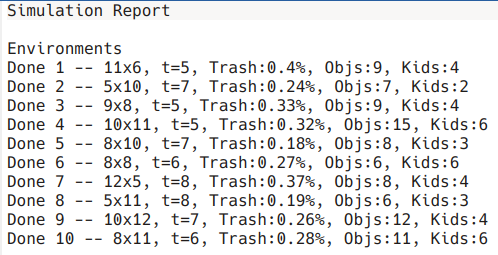
\includegraphics[scale=0.64]{./imgs/envs}
\end{figure}

Los valores resultantes para el modelo 1 el cual consideramos como un agente reactivo:

\begin{figure}[h]
	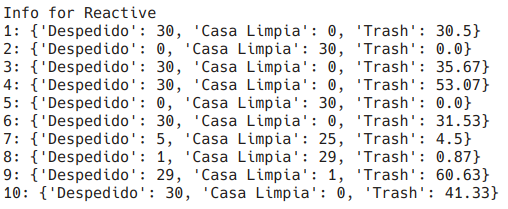
\includegraphics[scale=0.65]{./imgs/reactive}
\end{figure}

Y los valores para el segundo modelo el cual se considera proactivo

\begin{figure}[h]
	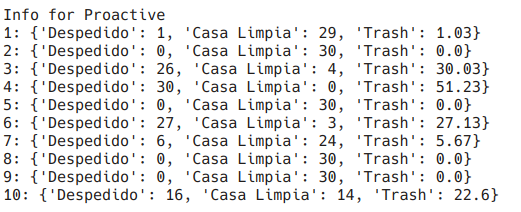
\includegraphics[scale=0.65]{./imgs/proactive}
\end{figure}

Para contrastar con estos resultados tambien se implementaron otros dos modelos como se vio anteriormente. Estos resultados pueden verse si se corre la simulacion definida en el archivo \verb|simulator.py|. El agente que busca como objetivo evitar el despido resulta muy malo para resolver el problema ya que siempre termina despedido debido a que es preferible iontentar ubicar a los ni\~nos primeramente sin tener en cuenta si esta acci\'on implica un aumento en la basura del ambiente. Este modelo se penso para corresponderse a la representaci\'on de $goal direct$ expresada en [2], pero los cambios cada $t$ turnos resultan perjudiciales para cualquier intento de crear una estrategia a largo plazo. El otra agente realiza la tarea m\'as pr\'oxima que tiene, ya sea buscar a un ni\~no, dejarlo en una cuna si es que lo carga y la tiene cerca o limpiar la basura cercana.

\section*{Repositorio}

\url{https://github.com/CRafa97/agent-simulation}

\begin{thebibliography}{9}
	[1] Temas de Simulaci\'on, Dr. Luciano Garc\'ia Garrido\\
	
	[2] Artificial Intelligence a 2020, Stuart Russell, Peter Norving
\end{thebibliography}

\label{end}

\end{document}

%===================================================================================
